\documentclass[a4]{article}

\usepackage[icelandic]{babel}
\usepackage[T1]{fontenc}
\usepackage{amsmath}
\usepackage{graphicx}
\usepackage{sidecap}
\usepackage[utf8]{inputenc}
\usepackage[left=1in,top=1in,right=1in,bottom=1in,nohead]{geometry}
\usepackage[framed,numbered,autolinebreaks,useliterate]{mcode}
\usepackage{amsfonts}
\usepackage{epstopdf}

\title{Töluleg Greining\\ Heimaverkefni 1}
\date{\today{}}
\author{ 
  Bjarki Geir Benediktsson,\and
  Haukur Óskar Þorgeirsson,\and
  Matthías Páll Gissurarson \and
  Kennari: Máni Maríus Viðarsson
  }



\begin{document}
\begin{flushright}
  Bjarki Geir Benediktsson,\\
  Haukur Óskar Þorgeirsson,\\
  Matthías Páll Gissurarson\\
\end{flushright}

\begin{center}
 \textsc{ \LARGE Töluleg Greining\\
  Heimaverkefni 1\\
  \today{}
  }
  \end{center}
\vfill

\maketitle
\section*{Inngangur}

Verkefni þetta snýst um að nota matlab til þess að leita að stöðupunktum í gefnu falli og flokka þá. fyrst með því að leita handvirkt með því að teikna kassa utan um mögulega stöðupunkta út frá jafnhæðarferlum fallsins, og hins vegar með því að leita skipulega fyrir innan gefinn ramma.

\section{Innlestur hnita frá mús}

Hér má sjá fyrsta forritið, en það má til dæmis keyra með \lstinline{square(-1,1,-1,1)} Til að keyra það á $[-1,1] \times [-1,1]$. Þetta forrit virkar þannig að það kemur upp mynd af hnitakerfi þar sem maður getur valið fjóra punkta með þvi að smella á hnitakerfið. Svo er teiknaður ferhyrningurinn sem punktarnir skilgreina (gefið að hann sé kúptur, annars kemur upp villa), og innan forritsins eru punktarnir komnir í þannig röð að þeir ganga réttsælis í ferhyrningnum. Forritið hættir ef smellt er á hægri músarhnapp.

\lstinputlisting[language=Matlab]{square.m}

Keyrt með \lstinline{square(-1,1,-1,1)} fæst:

\begin{figure}[h!]
\centering
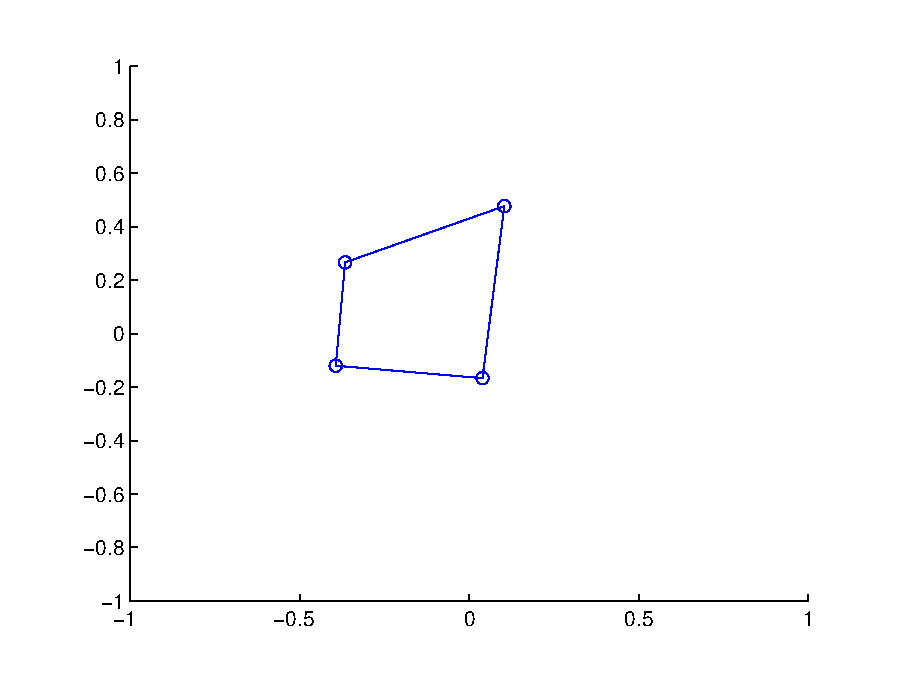
\includegraphics[width=0.7\textwidth]{squaredaemi.eps}
\caption{Ferhyrningur teiknaður}
\end{figure}

\begin{lstlisting}[language=Matlab]
ans =

  Columns 1 through 4

   -0.3664    0.1037    0.0392   -0.3940
    0.2661    0.4766   -0.1667   -0.1199

  Column 5

   -0.3664
    0.2661
\end{lstlisting}


\section{Er þessi punktur inni í þessum kassa?}

Hér er forrit sem vinnur meira á bak við tjöldin. Það reiknar, fyrir gefinn punkt (dálkvigur) og gefinn ferhyrning (gefinn með hornpunktunum sem eru raðaðir réttsælis) hvort punkturinn sé inni í ferhyrningnum.

\lstinputlisting[language=Matlab]{square_check.m}

Prufum að keyra þetta og dæla inn ferhyrning úr \lstinline{square} og núllpunktinum:

\begin{figure}[h!]
\centering
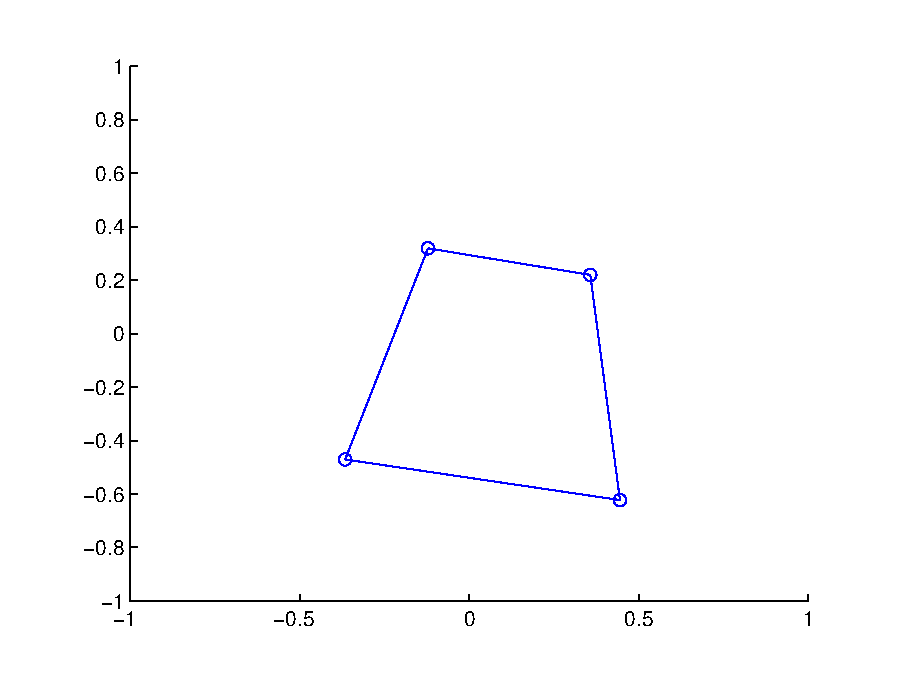
\includegraphics[width=0.7\textwidth]{sqchdaemi.eps}
\caption{Ferhyrningurinn sem var teiknaður (sjá má að núllpunkturinn er innan hans)}
\end{figure}

Úttak af skipanalínu MATLAB:

\begin{lstlisting}[language=Matlab]
>> square_check([0; 0],square(-1,1,-1,1))
:
ans =

     1
\end{lstlisting}

\section{}
Þetta forrit er forritið sem gerir mestu vinnuna, en það er forritið sem finnur fyrir okkur, með aðferð newtons, stöðupunkta fallsins. Það tekur inn
f:fallið sem á að athuga,
epsilon: sem tilgreinir skekkjuna frá réttum punkti sem við sættum okkur við,
$\Delta$ sem ákvarðar hversu lítill stigullinn má vera, það er\ hversu nákvæmlega þetta er stöðupunktur
og hversu nálægt Jacobi fylkið sem við erum að athuga er frá því að vera óandhverfanlegt,
en einnig hversu margar ítranir við viljum keyra, til að koma í veg fyrir að við lendum í óendanlegri lykkju.
Einnig má það taka inn endapunkta hnitakerfisins, en það er notað til þess að reikna út h1, sem notuð er  við nákvæmni í útreiknun á stigli og Jacobi fylki fallsins.

\lstinputlisting[language=Matlab]{newton_gradient.m}

Keyrsla með nokkrum dæmum. $\epsilon, \delta$ voru valin nógu lítil og $N$ nógu stórt þannig að forritið tæki ekki of langan tíma, en hinsvegar skilaði frekar nákvæmum niðurstöðum:

\lstinputlisting[language=Matlab]{newtongradientkeyrsla.m}
\begin{lstlisting}[language=Matlab]
ans =

     0
     0


ans =

     0
     0


ans =

  -1.570796327777076
                   0

\end{lstlisting}


\section{Handstýrð leit að stöðupunktum}

Nú erum við loks komin á þann stað að geta farið að leita að stöðupunktum. Forrit þetta teiknar fyrst upp jafnhæðarferla gefins falls og gefur svo kost á því að velja ferhyrning og svo byrjunarpunkt. Þá notar forritið \lstinline{newton_gradient} til að leita að stöðupunkti. Ef hann finnst er hann flokkaður, staðsetning og gildi hans skrifað út á úttakslínu og hann er merktur inn á myndina. Ef hann hann finnst ekki gerist ekkert. Svo er gefinn kostur á því að halda áfram og finna nýja stöðupunkta. Forritið hættir þegar smellt er á hægri músarhnapp.

\subsection*{Fallið f úr lið i}
\lstinputlisting[language=Matlab]{func.m}
\subsection*{Forritið}

Athugið að mcode virðist ekki styðja íslenska stafi, en útprentað er
``Hápunktur í'', ``Lágpunktur í'' og ``Söðulpunktur í'', ef punktur finnst,
en ``Ekki er hægt að segja til um (x,y) ='' ef ekki er hægt að segja til um punktinn.\\

\lstinputlisting[language=Matlab]{manualCriticalPointSearch.m}

\begin{figure}[h!]
\centering
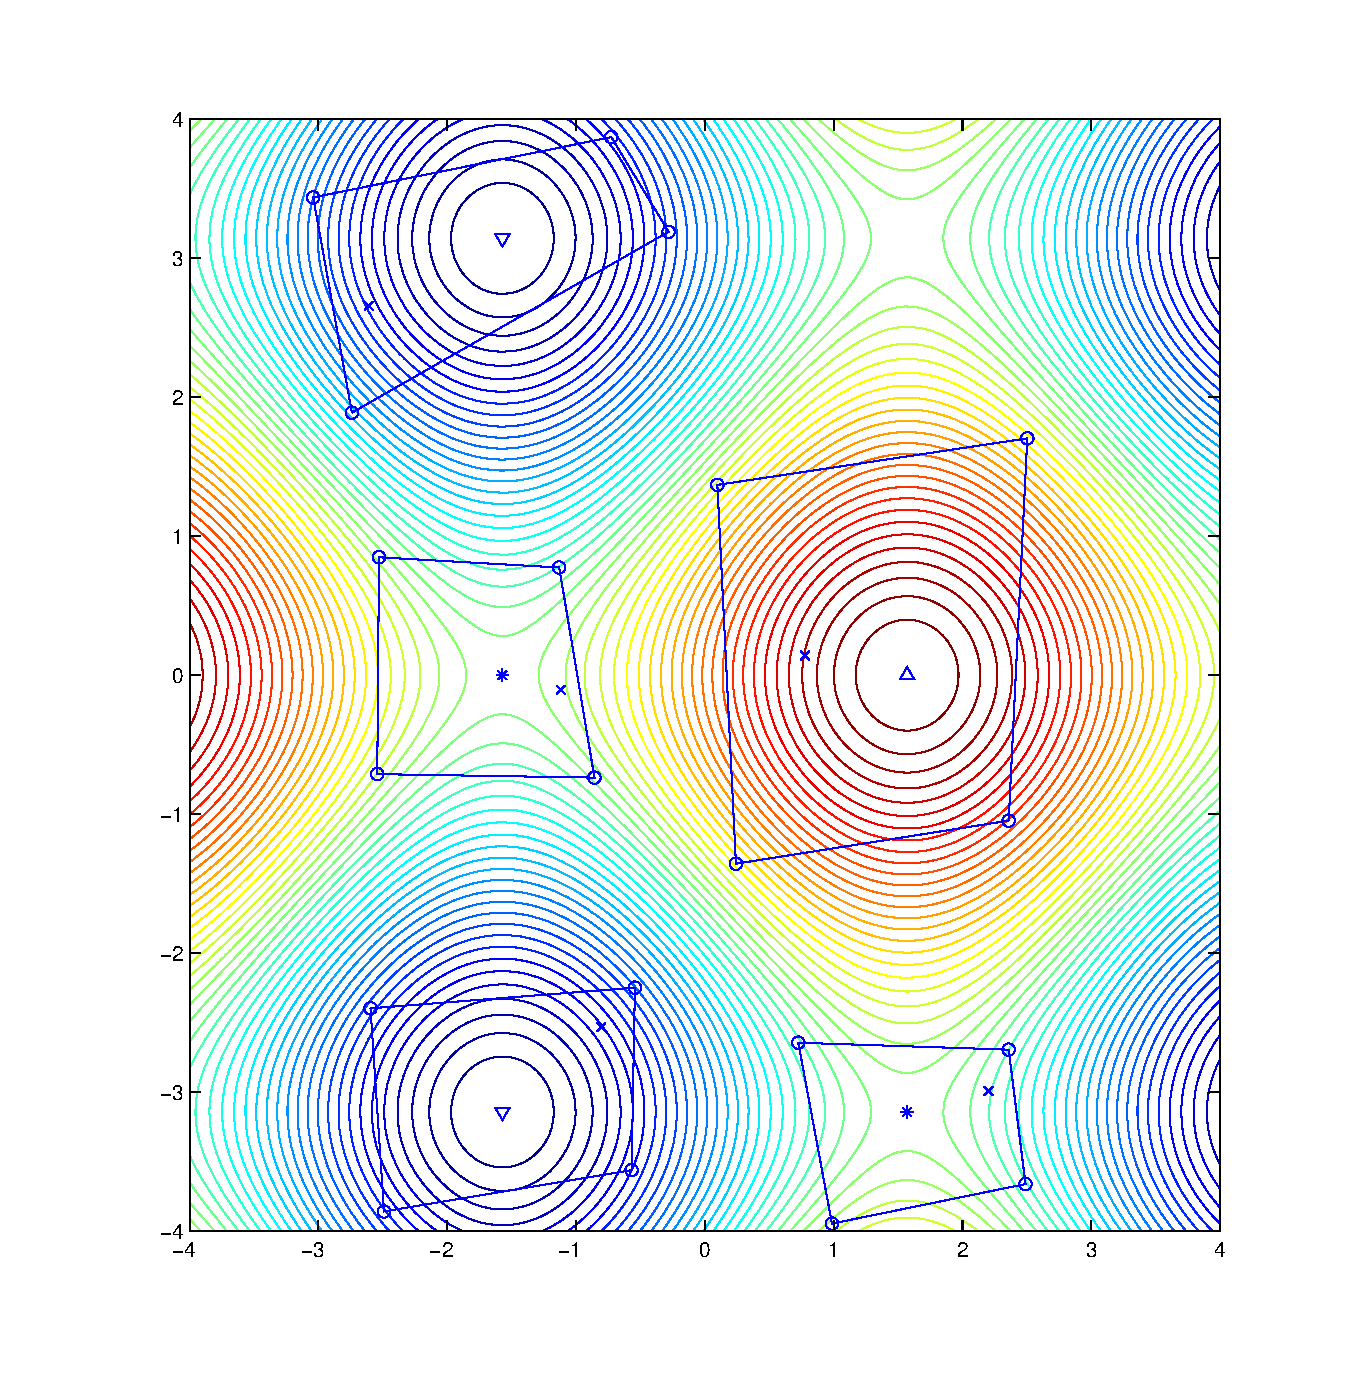
\includegraphics[width=0.7\textwidth]{manualdaemi1.eps}
\caption{Keyrsla á manual search}
\end{figure}

\newpage
Keyrsluskrá:
\lstinputlisting[language=Matlab]{manualcpkeyrsla.m}
Keyrsla, mynd má sjá á mynd 3.
\begin{lstlisting}[language=Matlab]
Hápunktur í (x,y) = (1.570796,-0.000000), f(x,y) = 2.000000
Söðulpunktur í (x,y) = (-1.570796,0.000000)
Lágpunktur í (x,y) = (-1.570796,3.141593), f(x,y) = -2.000000
Lágpunktur í (x,y) = (-1.570796,-3.141593), f(x,y) = -2.000000
Söðulpunktur í (x,y) = (1.570796,-3.141593)
\end{lstlisting}


\subsection*{}
Forrit sem skilgreinir
$$f(x)=\sum_{j=1}^N \alpha_j e^{-\frac{||x-q_j||^2}{\epsilon}$$
\lstinputlisting[language=Matlab]{func2.m}
Einnig er wrapper fyrir fallið, sem einfaldar notkun þess í forritinu. Athugið að ekki er hægt að senda fall inn í fall úr commandline í matlab nema að það sé anonymous.\\
\lstinputlisting[language=Matlab]{func2wrapper.m}

Forritið mætti vinna áfram og gera það t.d.\ sjálfvirkt, þannig mætti forða manni frá því að vera að tékka handvirkt, og auðvelda manni þannig vinnuna.
Einnig væri kannski sniðugt að láta það plotta í þrívídd, og sýna manni þannig að hágildi og lággildi eru í raun í punktunum, þ.e. að þar eru hápunktar og lágpunktar sléttunnar.

\section{Aukaliður}
Fall sem skiptir svæðinu öllu í reiti og leitar kerfisbundið að stöðupunktum
Fallið er keyrt á hliðstæðan hátt og handstýrða stöðupunktaleitin nema hvað bæta þarf inn fallgildinu boxes sem segir til um hve margar skiptingar á að gera á svæðinu á hvorn ás svo svæðinu er skipt í $boxes^2$ reiti og leitar innan hvers og eins reitar að sérstöðupunktum og flokkar þá sem hægt er.

\lstinputlisting[language=Matlab]{automaticCriticalPointSearch.m}

\begin{figure}[h!]
\centering
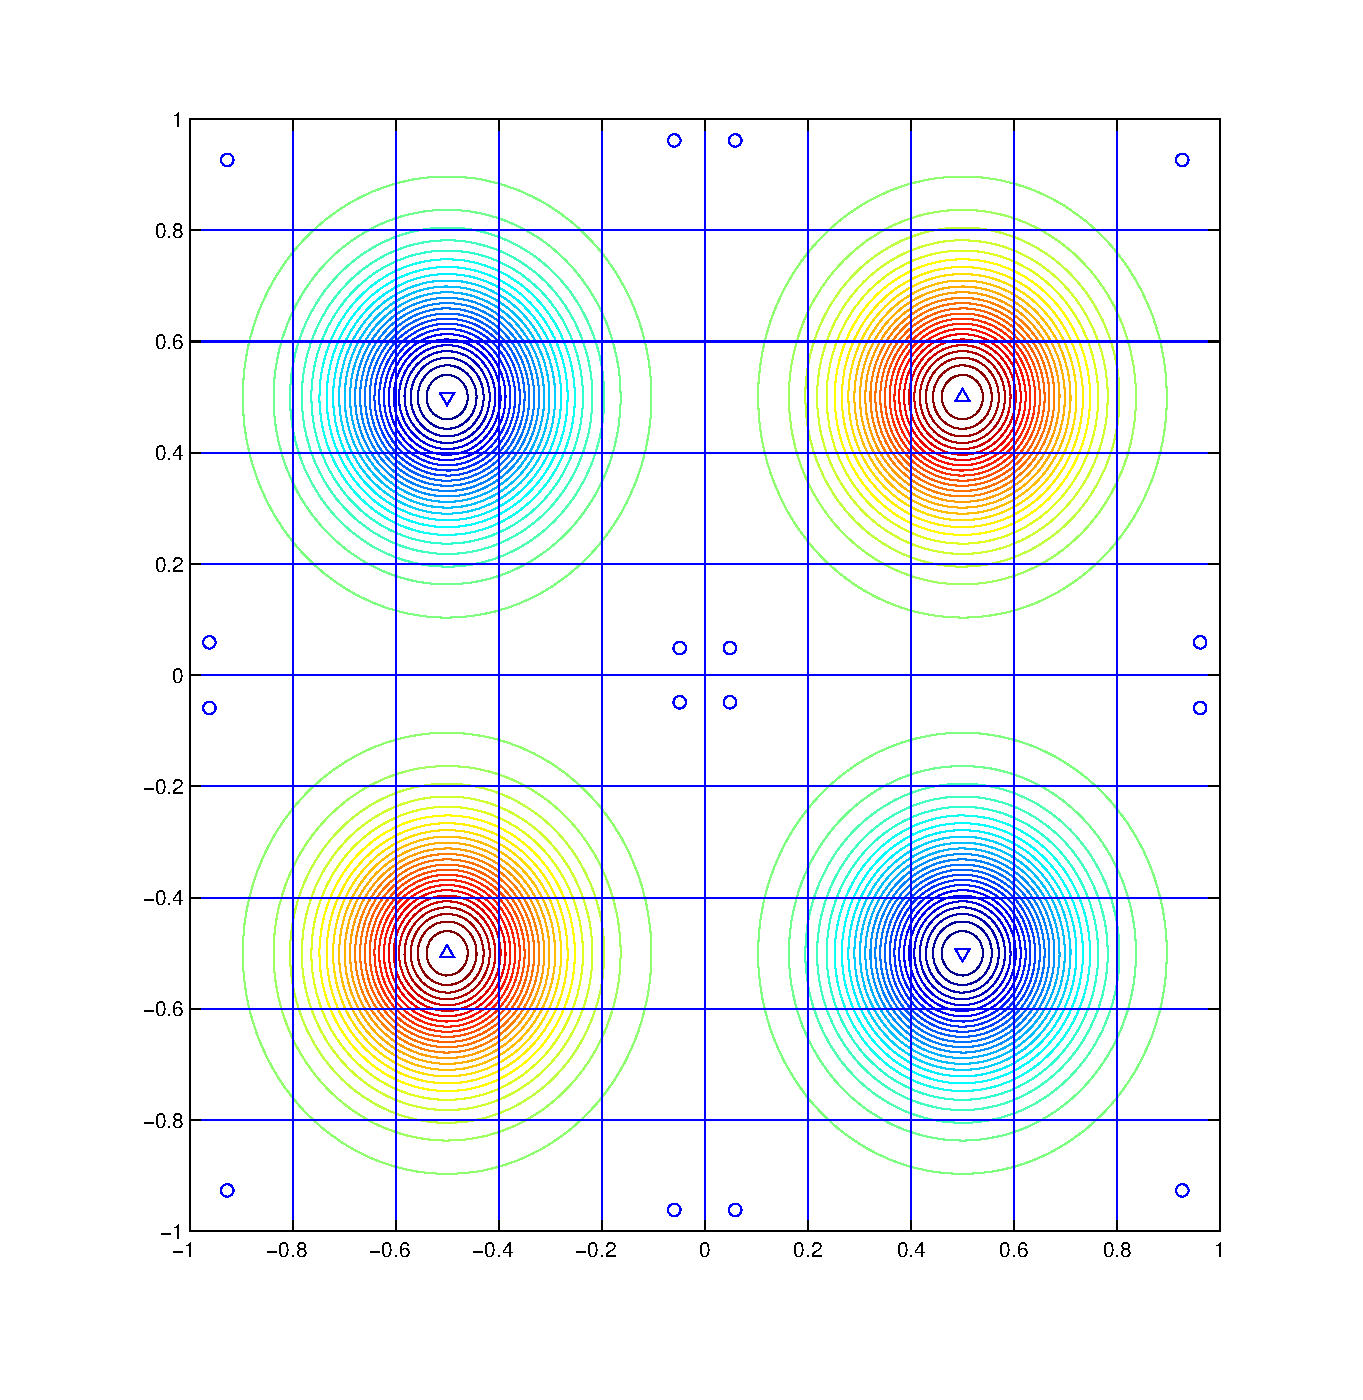
\includegraphics[width=0.7\textwidth]{acpkeyrsla1.eps}
\caption{Keyrsla á acpkeyrsla1}
\end{figure}

Keyrsluskrá acpkeyrsla1:
\lstinputlisting[language=Matlab]{acpkeyrsla1.m}

\newpage

Úttak keyrslu:
\begin{lstlisting}[language=Matlab]
Ekki hægt að segja til um (x,y) = (-0.926579,-0.926579)
Ekki hægt að segja til um (x,y) = (-0.961572,-0.058996)
Ekki hægt að segja til um (x,y) = (-0.961572,0.058996)
Ekki hægt að segja til um (x,y) = (-0.926579,0.926579)
Hápunktur í (x,y) = (-0.500000,-0.500000), f(x,y) = 1.000000
Lágpunktur í (x,y) = (-0.500000,0.500000), f(x,y) = -1.000000
Ekki hægt að segja til um (x,y) = (-0.058996,-0.961572)
Ekki hægt að segja til um (x,y) = (-0.048544,-0.048544)
Ekki hægt að segja til um (x,y) = (-0.048544,0.048544)
Ekki hægt að segja til um (x,y) = (-0.058996,0.961572)
Ekki hægt að segja til um (x,y) = (0.058996,-0.961572)
Ekki hægt að segja til um (x,y) = (0.048544,-0.048544)
Ekki hægt að segja til um (x,y) = (0.048544,0.048544)
Ekki hægt að segja til um (x,y) = (0.058996,0.961572)
Lágpunktur í (x,y) = (0.500000,-0.500000), f(x,y) = -1.000000
Hápunktur í (x,y) = (0.500000,0.500000), f(x,y) = 1.000000
Ekki hægt að segja til um (x,y) = (0.926579,-0.926579)
Ekki hægt að segja til um (x,y) = (0.961572,-0.058996)
Ekki hægt að segja til um (x,y) = (0.961572,0.058996)
Ekki hægt að segja til um (x,y) = (0.926579,0.926579)
\end{lstlisting}


\begin{figure}[h!]
\centering
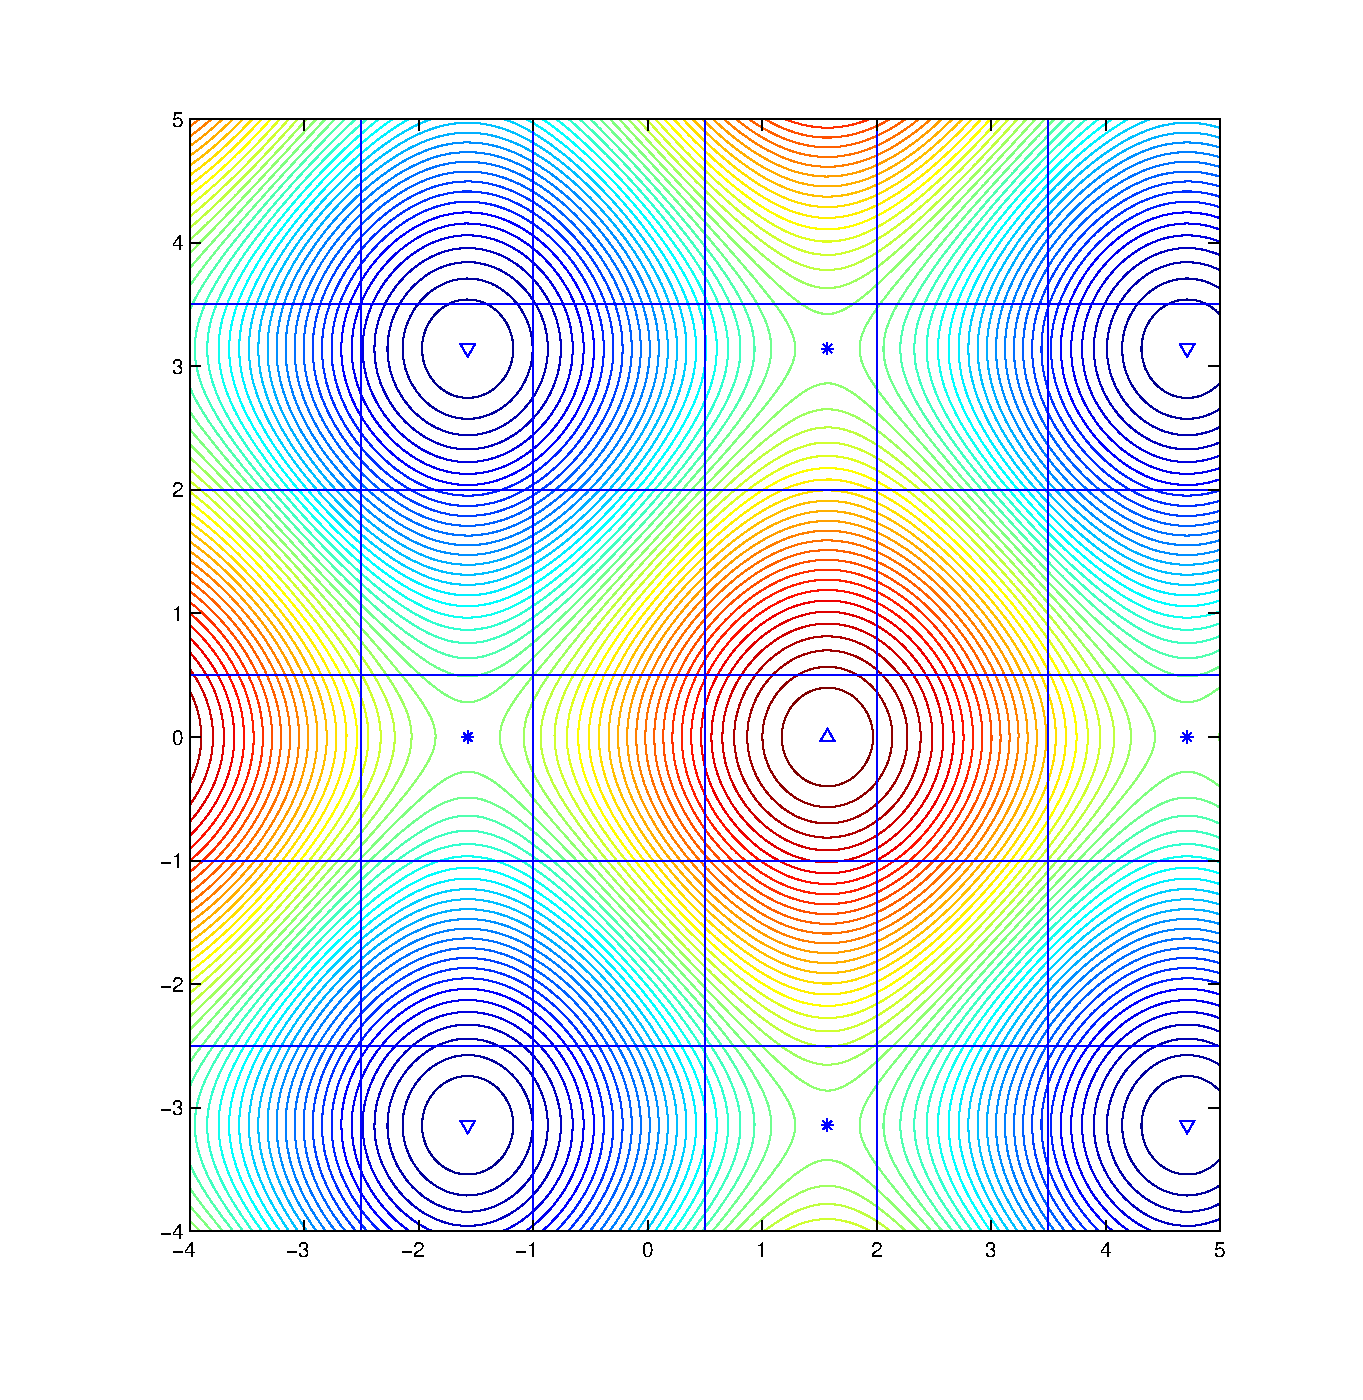
\includegraphics[width=0.7\textwidth]{acpkeyrsla2.eps}
\caption{Keyrsla á acpkeyrsla2}
\end{figure}

\newpage
Keyrsluskrá acpkeyrsla2:
\lstinputlisting[language=Matlab]{acpkeyrsla2.m}

Úttak keyrslu:
\begin{lstlisting}[language=Matlab]
Lágpunktur í (x,y) = (-1.570796,-3.141593), f(x,y) = -2.000000
Söðulpunktur í (x,y) = (-1.570796,0.000000)
Lágpunktur í (x,y) = (-1.570796,3.141593), f(x,y) = -2.000000
Söðulpunktur í (x,y) = (1.570796,-3.141593)
Hápunktur í (x,y) = (1.570796,0.000000), f(x,y) = 2.000000
Söðulpunktur í (x,y) = (1.570796,3.141593)
Lágpunktur í (x,y) = (4.712389,-3.141593), f(x,y) = -2.000000
Söðulpunktur í (x,y) = (4.712389,0.000000)
Lágpunktur í (x,y) = (4.712389,3.141593), f(x,y) = -2.000000
\end{lstlisting}


\vspace{20 mm}
Að skýrsluni unnu :
\hspace{0.5cm} \makebox[1.5in]{\hrulefill}
\hspace{0.5cm} \makebox[1.5in]{\hrulefill}
\hspace{0.5cm} \makebox[1.5in]{\hrulefill}
\end{document}
